\documentclass[11pt, letterpaper, twoside]{article}
\usepackage{geometry}
\usepackage[utf8]{inputenc}
\usepackage[english]{babel}
\usepackage[runin]{abstract}
\usepackage{titling}
\usepackage{booktabs}
\usepackage{fancyhdr}
\usepackage{helvet}
\usepackage{csquotes}
\usepackage{graphicx}
\usepackage{blindtext}
\usepackage{parskip}
\usepackage{etoolbox}
\usepackage{amsmath}
\usepackage{float}
\usepackage{hyperref}

\input{preamble.tex}

\title{\textbf{Frequency-Domain Object Detection and Counting Using Fourier Cross-Correlation}}
\author{Mohammed Ayaan \\ 100920102 \and Jacob Mendler \\ 100911093}
\runningtitle{Fourier Cross-Correlation for Object Detection}
\runningauthor{Jacob Mendler and Mohammed Ayaan}
\affiliation{Ontario Tech University}
\department{Faculty of Science, Computer Science}
\memoid{CSCI 4220U}
\theyear{2026}
\mydate{April 10, 2026}

\begin{document}

\maketitle

\begin{abstract}
\noindent
This project develops and evaluates an object detection and counting pipeline for repeated objects in images. Our initial proposal was to build on Fourier cross-correlation and extend it with stronger robustness to rotation and scale. In the final implementation, we compare the original Lab 3 Fourier cross-correlation baseline against an improved detector that uses multi-scale and multi-angle template matching, circular masking, and duplicate suppression. The system is evaluated on a dataset of coin images with ground truth annotations. Results show that the improved method substantially reduces false positives and improves overall detection quality, although it remains sensitive to template choice and still fails in some challenging cases. This design choice allows us to explore the practical limits of template-based detection methods in real-world conditions.
\end{abstract}

\vspace{2.5cm}

\thispagestyle{firstpage}

\pagebreak

\newgeometry{}

\section{Introduction}

Object detection and counting are fundamental problems in computer vision. In this project, we focus on detecting repeated objects, specifically coins, using template-based matching methods.

The original goal of the project was to extend Fourier cross-correlation for more robust detection under variations in scale and rotation. Over the course of development, the project evolved into a comparison between a baseline frequency-domain method from Lab 3 and a significantly improved detector that incorporates multi-scale and multi-rotation matching, template masking, and duplicate suppression.

The objective is to evaluate how these improvements affect detection accuracy and robustness on a realistic dataset. While these improvements significantly enhance detection performance, they also introduce new tradeoffs and limitations that must be carefully analyzed.

An important design decision in this project was to focus on template-based methods rather than modern deep learning approaches such as YOLO. While they would achieve higher performance, we wanted to test how far such methods could go.

\section{Background}

Fourier cross-correlation allows efficient template matching:

\begin{equation}
C(x, y) = \mathcal{F}^{-1}\left(\mathcal{F}(I)\cdot \overline{\mathcal{F}(T)}\right)
\end{equation}
where $I$ is the input image, $T$ is the template, and $\mathcal{F}$ denotes the Fourier transform. Peaks in the resulting correlation map indicate locations where the template closely matches the image.

While this formulation enables efficient template matching, it assumes that the object appears at the same scale and orientation as the template. In real-world images, this assumption rarely holds, especially for objects such as coins that can appear rotated and scaled differently. This limitation motivates the need for extensions that account for scale and rotation variation, which form the basis of the improved detection method used in this project.

\section{Methodology}

\subsection{Baseline Method}

The baseline method directly follows the Lab 3 implementation. It performs frequency-domain cross-correlation using a single fixed template and detects peaks in the resulting correlation map corresponding to likely object locations. Although it is computationally efficient, it lacks robustness to variations in scale, rotation and background noise.

\subsection{Improved Method}
These components are applied sequentially as part of a unified detection pipeline, where template matching is performed across scales and rotations, responses are aligned and aggregated, and final detections are filtered to remove duplicates. The improved detector introduces several major enhancements:

\subsubsection{Thresholding}

Correlation responses are filtered using a threshold to retain only strong matches. This step plays a critical role in reducing false positives but also contributes to missed detections when valid matches fall below the threshold.

\subsubsection{Multi-Scale Matching}
The template is resized across a range of scales between 0.25 and 1.25 to account for different object sizes.

\subsubsection{Rotation Handling}
The template is rotated at multiple angles (0 to 360 degrees in 30-degree steps), allowing detection of arbitrarily oriented coins.

\subsubsection{Circular Masking}
A circular mask is applied to the template to focus on the coin shape and remove background influence.

\subsubsection{Aligned Correlation Mapping}
A key improvement is correcting the coordinate alignment when using rotated templates. The correlation responses are mapped back into a consistent coordinate system before aggregation, ensuring accurate localization.

\subsubsection{Duplicate Suppression}
Instead of traditional non-maximum suppression, the algorithm uses a center-based filtering approach. Detections are accepted only if their center does not fall inside an already confirmed detection, reducing duplicate detections.

\subsubsection{Scale Ordering}
Detection is performed from largest to smallest scale, ensuring that large objects are detected first and preventing smaller-scale detections from overwriting correct large detections.

\subsection{Evaluation}

Detections are evaluated using Intersection over Union (IoU), with a threshold of 0.3 to determine whether a predicted bounding box matches a ground truth object. This relatively low threshold accounts for minor localization errors introduced by scaling and rotation. Meanwhile, performance is measured using precision, recall, and F1 score. Precision measures the proportion of correct detections among all detections, recall measures the proportion of true objects detected, and F1 score provides a balanced measure of both.

\section{Dataset}

The dataset consists of 63 coin images with ground truth bounding boxes. The images include variations in scale, rotation, lighting, and background complexity. These variations make the dataset more challenging than the controlled examples used in the original lab, and provide a more realistic test of the detection pipeline. In particular, the presence of scale and rotation variation directly motivates the need for multi-scale and multi-angle matching, while background clutter increases the likelihood of false positives in simpler methods.
\section{Results}

\subsection{Aggregate Performance}

Based on all 63 images in the dataset, these values are computed as averages across them with the improved method achieving:

\begin{itemize}
    \item Precision: 0.82
    \item Recall: 0.56
    \item F1 Score: 0.64
\end{itemize}

The baseline method achieved:

\begin{itemize}
    \item Precision: 0.18
    \item Recall: 0.43
    \item F1 Score: 0.25
\end{itemize}

These results show that the improved detector significantly outperforms the baseline in precision and overall F1 score. A key observation is that the improved method frequently achieves near-perfect precision when detections are successful, but also exhibits complete detection failures in some cases, which reduces overall recall.

\subsection{Qualitative Results}
The following examples are selected directly from the evaluated dataset and correspond to representative behaviors observed in the full results, including ideal detection, false-positive suppression, and challenging failure cases.

\begin{figure}[hbtp]
\centering
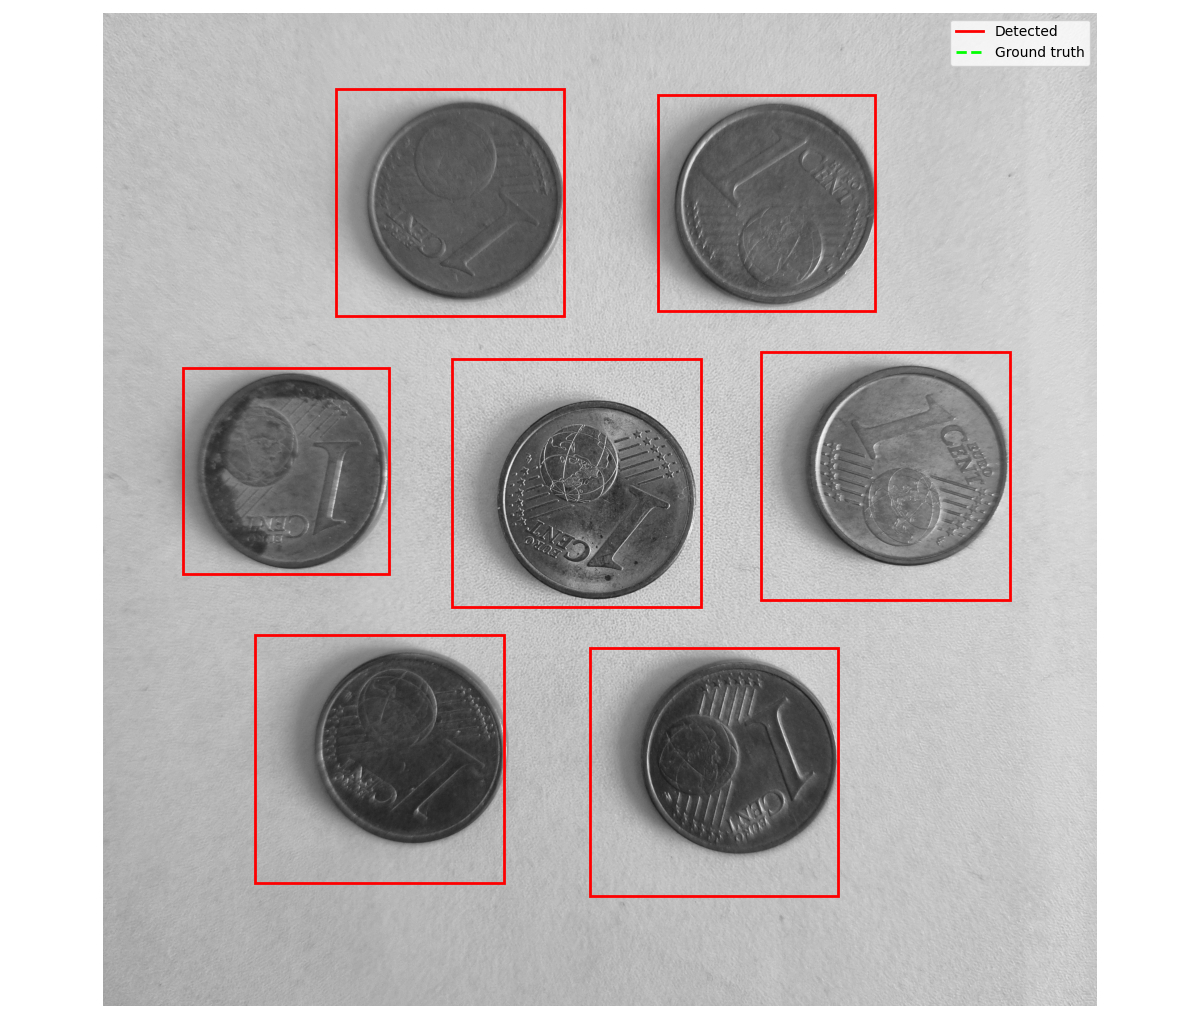
\includegraphics[width=0.48\textwidth]{new_151117.png}
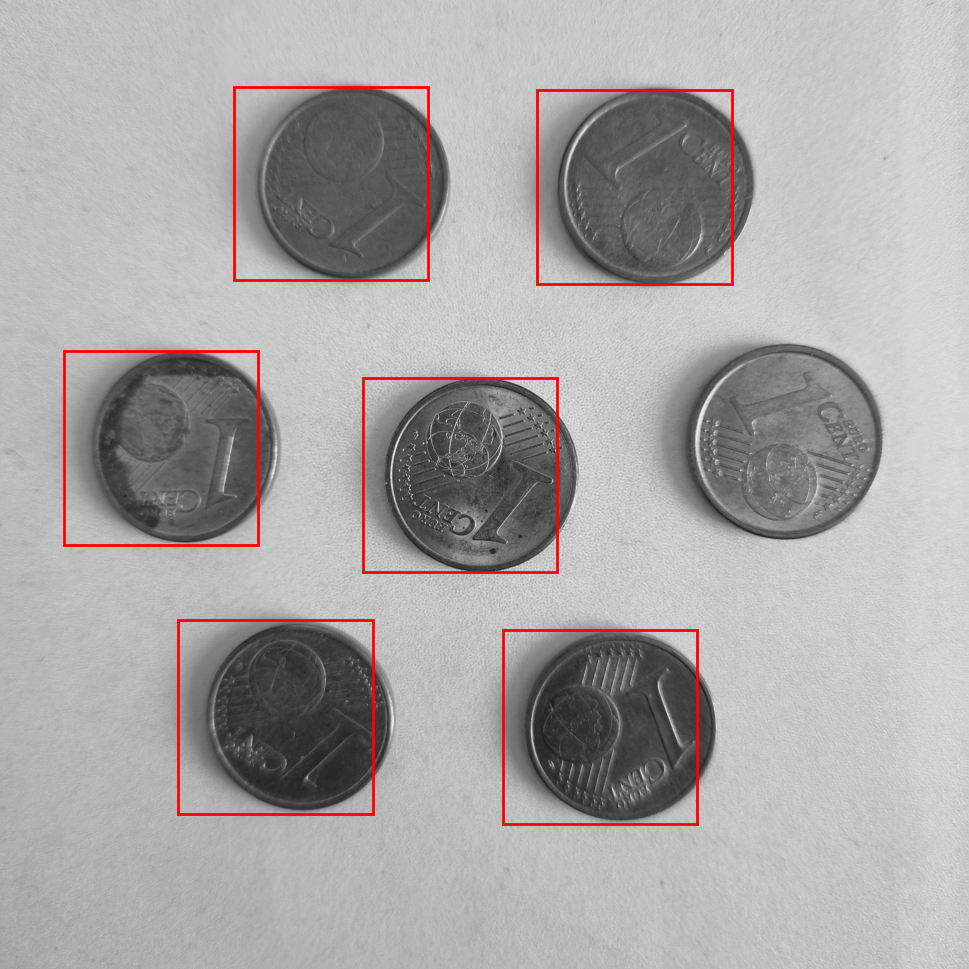
\includegraphics[width=0.48\textwidth]{baseline_151117.png}
\caption{Improved vs baseline detection for image 20210324\_151117.
The improved method correctly detects all coins with clean bounding boxes, while the baseline slightly under-detects.}
\end{figure}

\begin{figure}[hbtp]
\centering
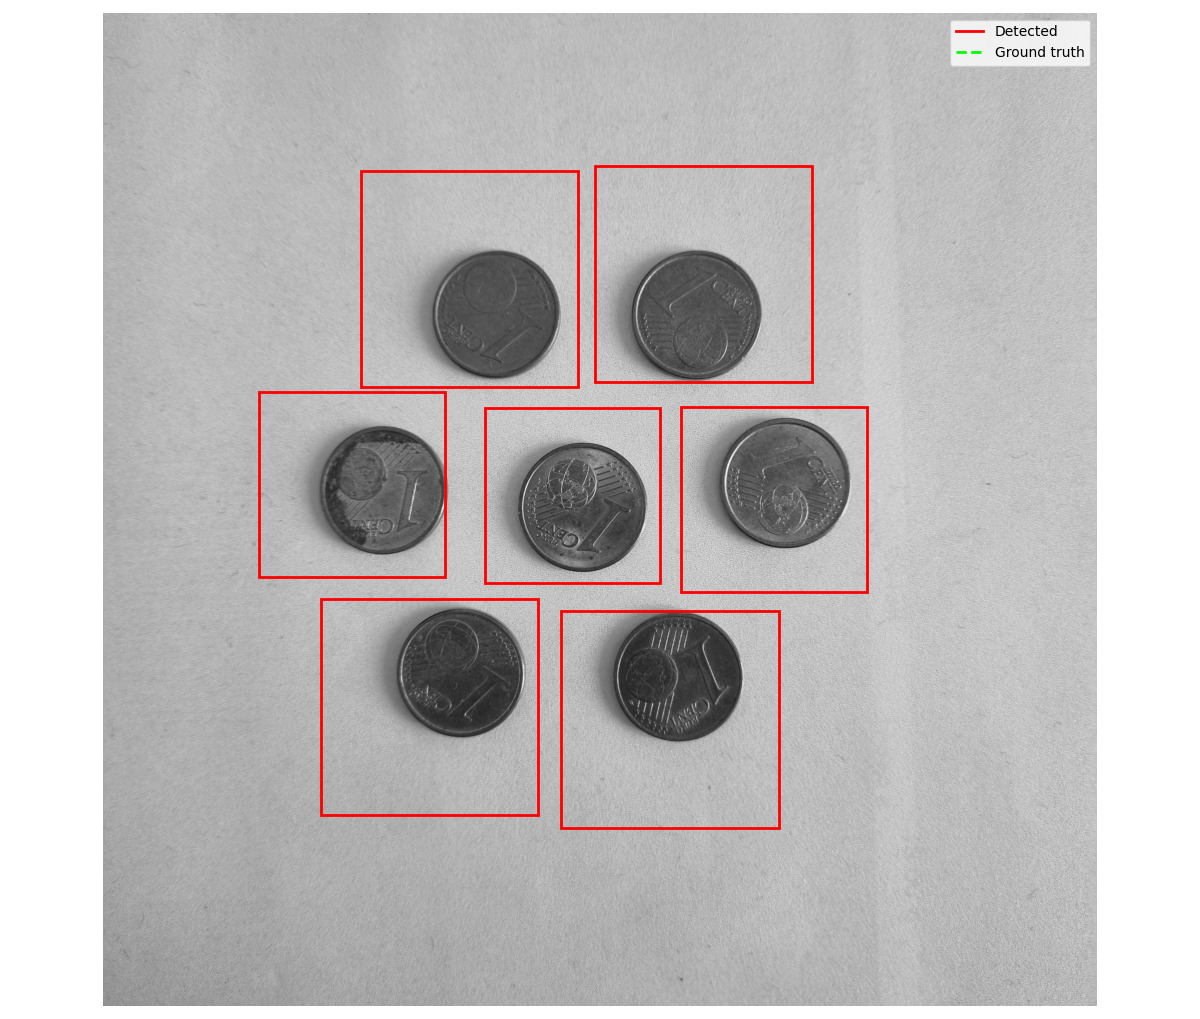
\includegraphics[width=0.48\textwidth]{new_151121.png}
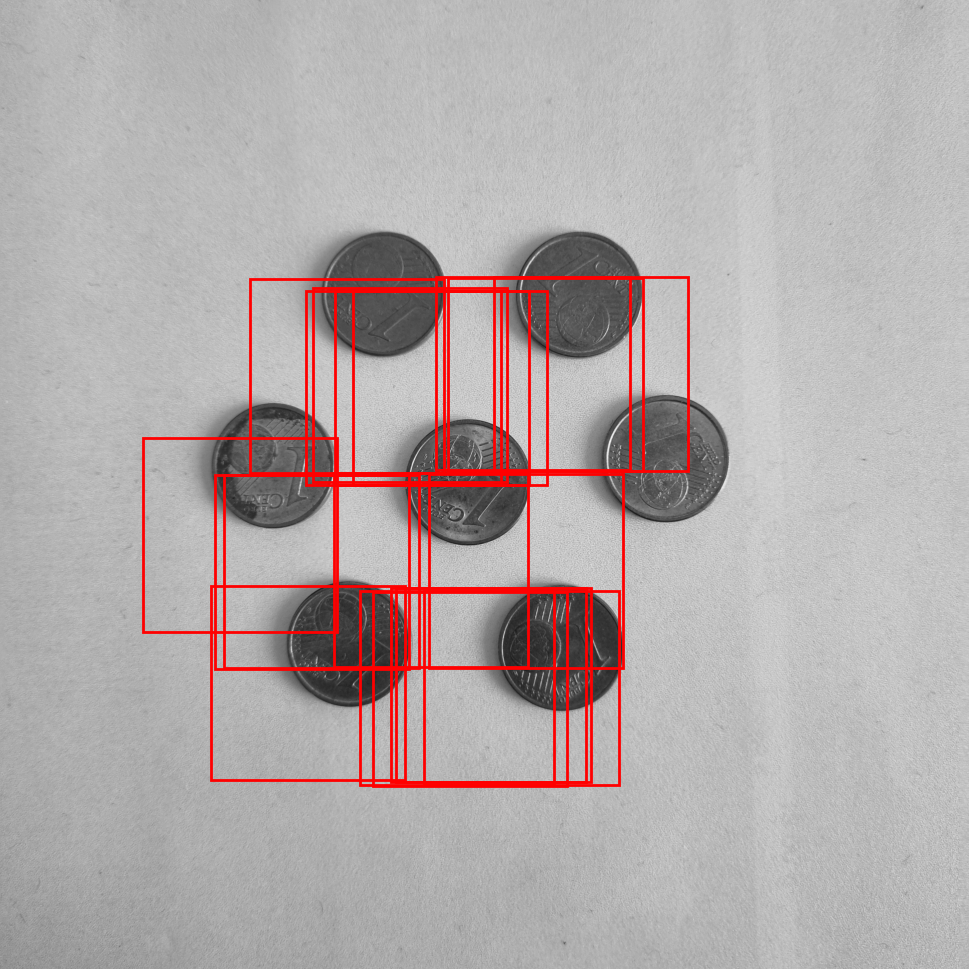
\includegraphics[width=0.48\textwidth]{baseline_151121.png}
\caption{Improved vs baseline detection for image 20210324\_151121.
The baseline produces many false positives, while the improved method detects all coins correctly.}
\end{figure}

\begin{figure}[hbtp]
\centering
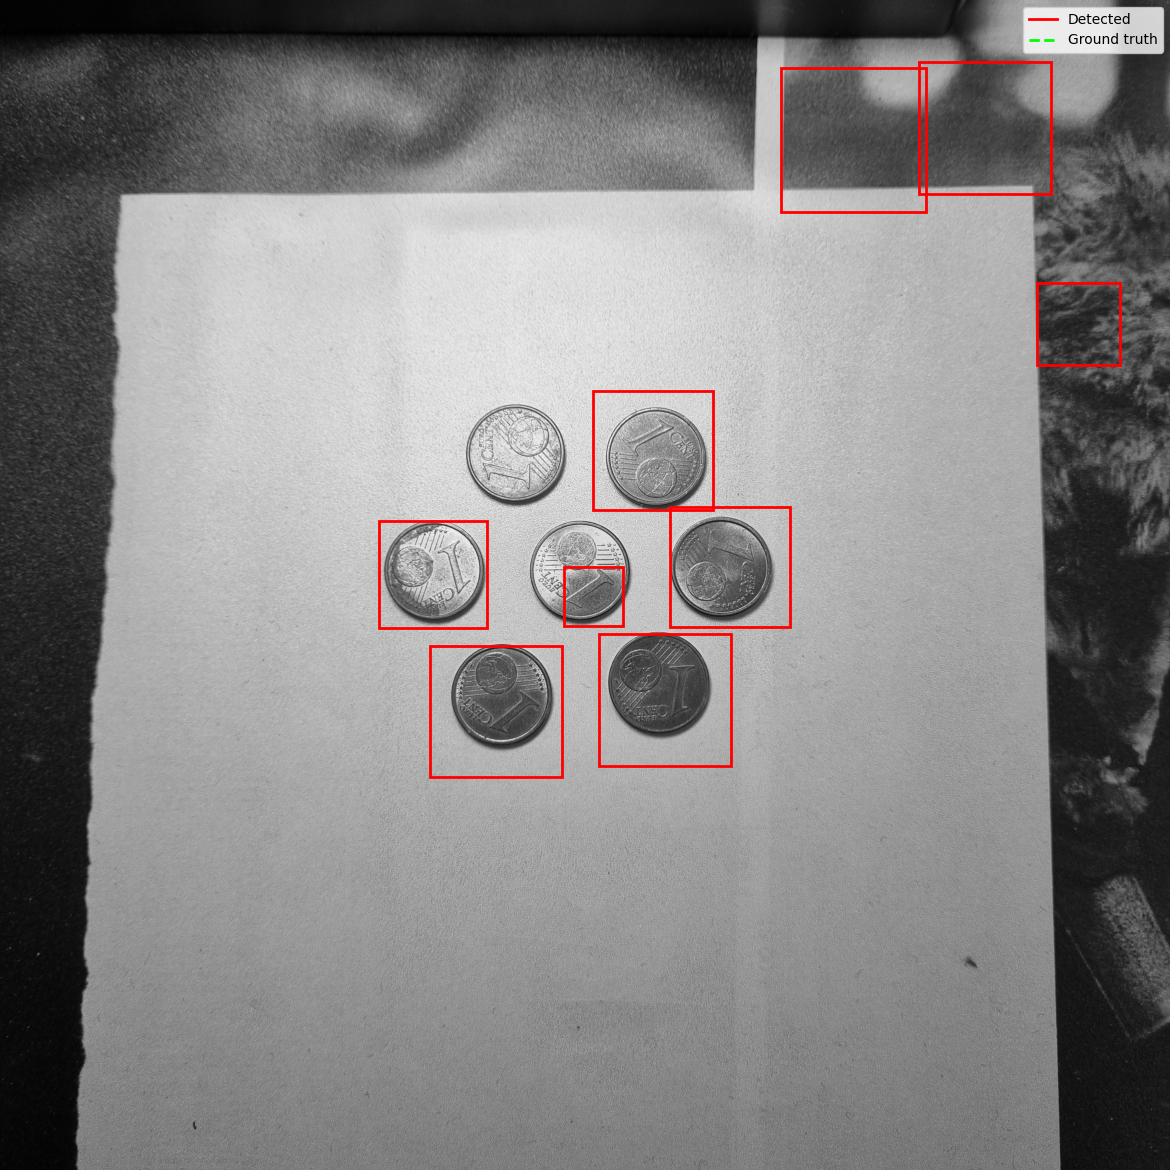
\includegraphics[width=0.48\textwidth]{new_151304.png}
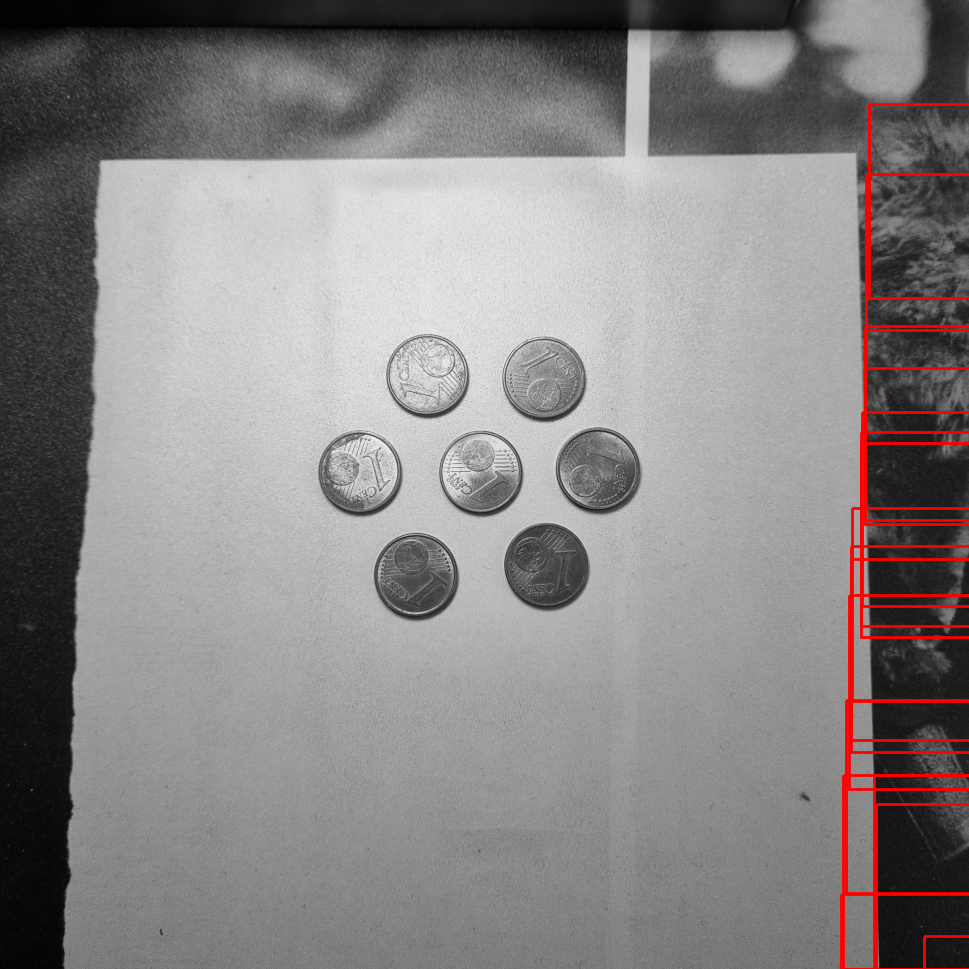
\includegraphics[width=0.48\textwidth]{baseline_151304.png}
\caption{Improved vs baseline detection for image 20210324\_151304.
This is a hard case example, the improved method detects several coins with fewer false positives, while the baseline produces many incorrect detections.}
\end{figure}

\begin{figure}[hbtp]
\centering
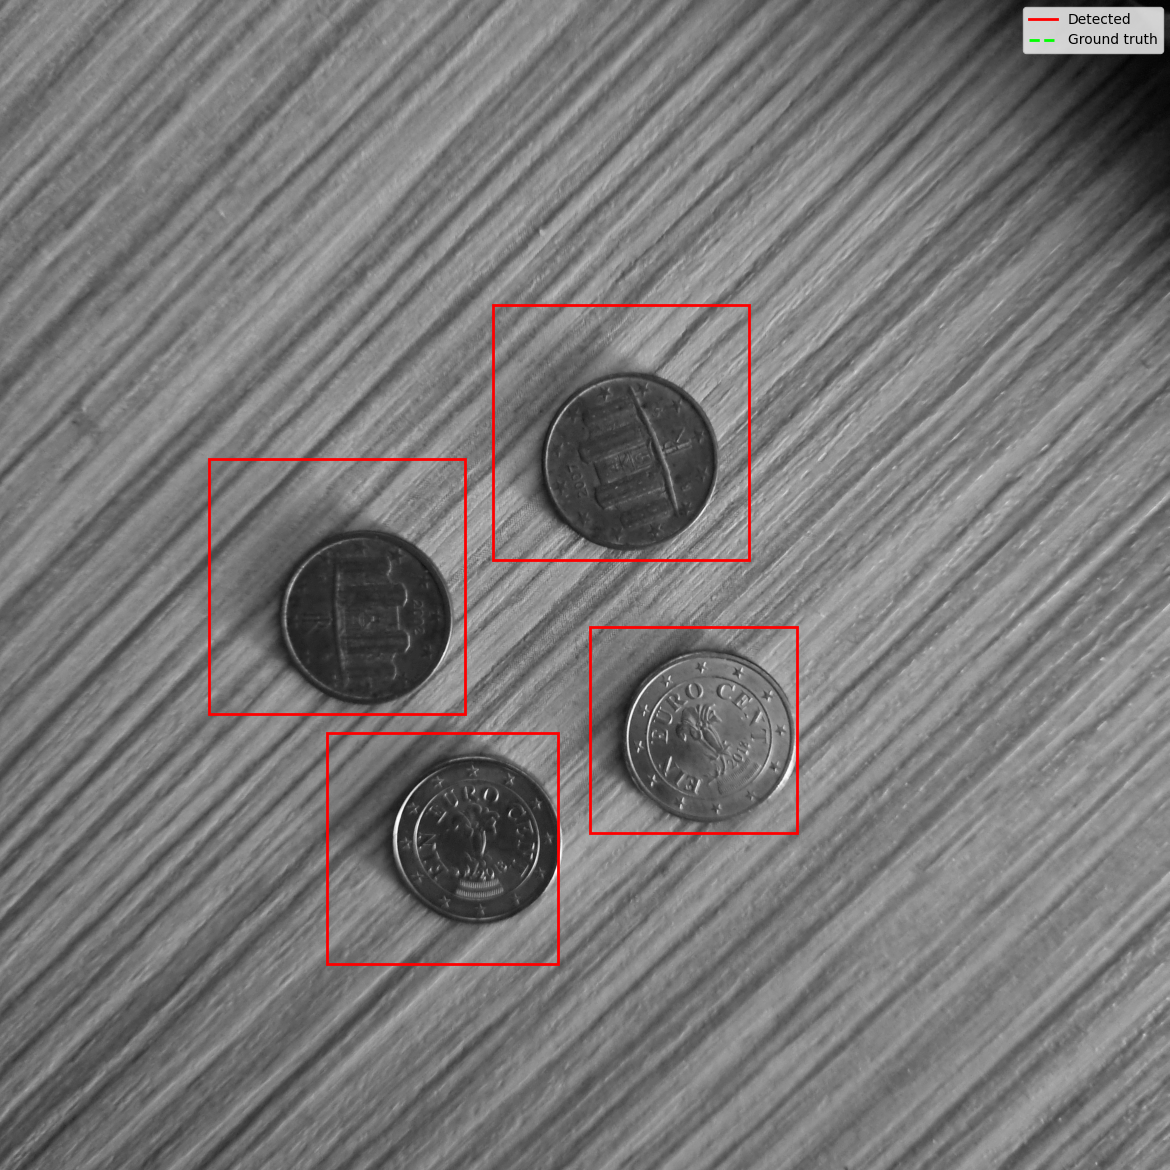
\includegraphics[width=0.48\textwidth]{new_161615.png}
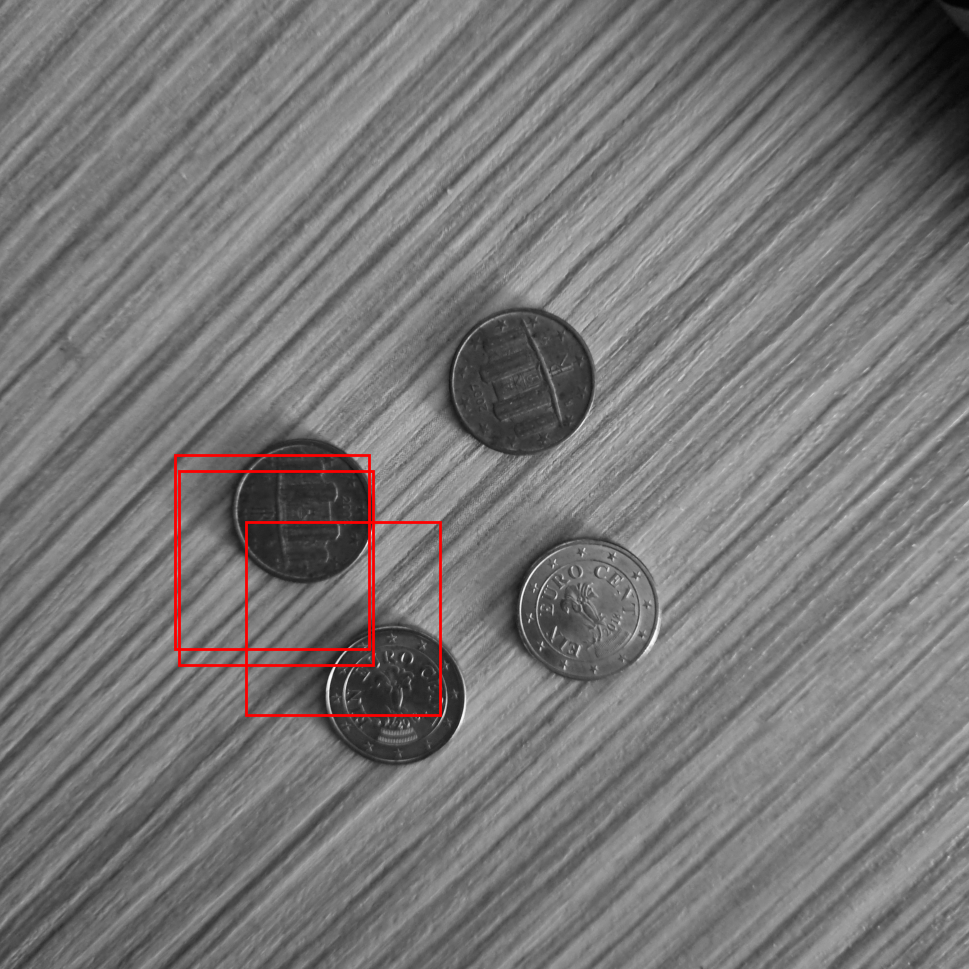
\includegraphics[width=0.48\textwidth]{baseline_161615.png}
\caption{Improved vs baseline detection for image 20210328\_161615.
Both methods detect objects, but the improved method produces cleaner and more accurate bounding boxes.}
\end{figure}

\FloatBarrier

\section{Discussion}

The improved detector demonstrates a clear advantage over the baseline method, particularly in precision. The baseline frequently produces excessive false positives due to strong correlation responses in irrelevant regions. This behavior is consistent with the quantitative results, where the improved method achieves significantly higher precision but exhibits reduced recall.

The baseline method produces false positives because strong correlation responses can occur in regions that partially resemble the template, even when no true object is present. The improved method addresses this issue through multi-scale matching, rotation handling, and duplicate suppression. These additions significantly reduce false detections and improve overall reliability. 

However, this improvement introduces a clear tradeoff. The improved detector is more conservative and, in many cases, fails to detect any objects at all. These complete detection failures contribute significantly to the reduction in recall and highlight the sensitivity of template matching to factors such as lighting variation, background clutter, and mismatch between the template and target objects.

This precision-recall tradeoff is one of the most important findings of the project. In practical applications, high precision is often more desirable than high recall, making the improved method more useful despite its limitations.

Additionally, the improved method is computationally expensive due to exhaustive scale and rotation search.

These results also reflect the fundamental limitations of template matching approaches. While enhancements such as multi-scale and multi-rotation search improve robustness, the method still relies heavily on the similarity between the template and target objects. This makes it inherently less adaptable than learning-based methods, but valuable for understanding the core mechanics of object detection.

\section{Conclusion}

This project demonstrates that extending a basic template-matching pipeline with practical enhancements can significantly improve detection performance. The improved method achieves substantially higher precision and better overall detection quality compared to the baseline, although challenges remain in recall and computational efficiency. This project successfully demonstrates both the strengths and limitations of template-based detection, providing insight into how far classical methods can be extended before more advanced approaches become necessary. Overall, the results highlight the importance of robustness mechanisms in real-world object detection systems.

\section{Code Repo}
https://github.com/Jazoe/Frequency-Domain-Object-Detection-and-Counting-Using-Fourier-Cross-Correlation

\end{document}